% Straight up stealing preamble from Eli Holmes 
%%%%%%%%%%%%%%%%%%%%%%%%%%%%%%%%%%%%%%START PREAMBLE THAT IS THE SAME FOR ALL EXAMPLES
\documentclass{article}

%Required: You must have these
\usepackage{Sweave}
\usepackage{graphicx}
\usepackage{tabularx}
\usepackage{hyperref}
\usepackage{natbib}
\usepackage{pdflscape}
\usepackage{array}
\usepackage{gensymb}
%\usepackage[backend=bibtex]{biblatex}
%Strongly recommended
  %put your figures in one place
%\SweaveOpts{prefix.string=figures/, eps=FALSE} 
%you'll want these for pretty captioning
\usepackage[small]{caption}

\setkeys{Gin}{width=0.8\textwidth}  %make the figs 50 perc textwidth
\setlength{\captionmargin}{30pt}
\setlength{\abovecaptionskip}{10pt}
\setlength{\belowcaptionskip}{10pt}
% manual for caption  http://www.dd.chalmers.se/latex/Docs/PDF/caption.pdf

%Optional: I like to muck with my margins and spacing in ways that LaTeX frowns on
%Here's how to do that
 \topmargin -1.5cm        
 \oddsidemargin -0.04cm   
 \evensidemargin -0.04cm  % same as oddsidemargin but for left-hand pages
 \textwidth 16.59cm
 \textheight 21.94cm 
 %\pagestyle{empty}       % Uncomment if don't want page numbers
 \parskip 7.2pt           % sets spacing between paragraphs
 %\renewcommand{\baselinestretch}{1.5} 	% Uncomment for 1.5 spacing between lines
\parindent 0pt% sets leading space for paragraphs
\usepackage{setspace}
%\doublespacing

%Optional: I like fancy headers
%\usepackage{fancyhdr}
%\pagestyle{fancy}
%\fancyhead[LO]{How do climate change experiments actually change climate}
%\fancyhead[RO]{2016}
 
%%%%%%%%%%%%%%%%%%%%%%%%%%%%%%%%%%%%%%END PREAMBLE THAT IS THE SAME FOR ALL EXAMPLES

%Start of the document
\begin{document}

%\SweaveOpts{concordance=TRUE}
 \bibliographystyle{..//..//refs/bibstyles/amnat.bst}
\title{Spatial and temporal shifts in photoperiod with climate change} % perspective paper for OSPREE analyses

\author{A.K. Ettinger, D. Buonaiuto, C. Chamberlain, I. Morales-Castilla, E. Wolkovich}
%\date{\today}
\maketitle  %put the fancy title on
%\tableofcontents      %add a table of contents
%\clearpage
%goal is NCC Perspective
%Need to submit "brief synopsis through our online submission system before preparing a manuscript for formal submission. The synopsis should outline the topics that will be covered, list any recent, key publications in the area, and state the last time the topic was reviewed (if it has been reviewed previously)."
%should be presented using simple prose, avoiding excessive jargon and technical detail.
%3,000–5,000 words and typically include 4–6 display items (figures, tables or boxes). (we have 6)
%up to 100 references; citations should be selective. (we have 83 now)
%%%%%%%%%%%%%%%%%%%%%%%%%%%%%%%%%%%%%%%%%%%%%%%%%%%

%%%%%%%%%%%%%%%%%%%%%%%%%%%%%%%%%%%%%%%%%%%%%%%%%%%

\section*{Summary}
Climate change causes both temporal and geographic shifts in species that affect the daylength (photoperiod) that they experience. Photoperiod is a common trigger of seasonal biological responses (e.g., it affected phenology in 84\% of studies that manipulated photoperiod i woody plants). However, it has not been a focus of climate change forecasting to date, especially for early-season (`spring') events---which are often thought to be driven by temperature. Here we address the potential for current knowledge of photoperiod responses to be incorporated into attempts to forecast the spatial-temporal distribution of biodiversity. We find that impacts on experienced photoperiod due to temporal shifts will be orders of magnitude larger than impacts due to spatial shifts (e.g., 1.6 hours change versus a minute). Incorporating photoperiod into forecasts may be possible for some species by leveraging existing experimental data; for example, growth chamber experiments on woody plant spring phenology often have data relevant for climate change impacts. We highlight how new modelling approaches to improve predictions of when, where, and how much photoperiod is likely to affect future spring phenology, combined with new empirical work to identify and understand biogeographic and phenotypic variation in photoperiod, could rapidly advance our understanding. %currently 197 words

% How does it act as a cue, how wrong are forecasts and is there predictable variation? (Traits etc.) 

\section*{Introduction}
\par Shifts in the timing of spring events --- including flowering, bird arrival, egg hatching and a myriad of other biological activities --- are some of the most widely documented signals of climate change. Across taxa from plants and insects to mollusks and mammals, spring phenology is occurring earlier as temperatures warm, with average shifts of 1.2 to 5.1 days earlier per decade \citep{bradley1999,parmesan2003, root2003} or 1.3 to 5.6 days earlier per \degree C of warming \citep{Wolkovich:2012n,polgar2013}. Indeed, early spring phenology is shifting more rapidly than later season phenology in many cases \citep{bradley1999,menzel2006}, suggesting strong temperature sensitivity of spring phenophases.

\par Spring phenology is not controlled solely by temperature, however. Photoperiod is also a critical cue for plants and animals, signaling changes in growth, mating, and reproduction across diverse species \citep[e.g.,][]{Howe:1996,flynn2018,solbakken1994,mcallan2006,lagercrantz2009}. Photoperiod is used to synchronize activities with seasonal climatic changes \citep[e.g.,][]{Hsu:2011,Singh:2017,Basler:2012} because it is consistent across years, especially compared to other seasonal cues such as temperature and precipitation \citep{saikkonen2012}. For example, relying on photoperiod, rather than temperature alone, may prevent woody plants from leafing out during ``false spring" events \citep[unusually warm periods during winter that are followed by a return of cold temperatures][] {Gu2008}. With current rapid warming, however, photoperiod may also potentially slow advancing spring phenology. 

\par Recent studies offer inconsistent views about whether photoperiod may eventually restrict advances in spring phenology in a warmer world. Some studies suggest that, with additional warming, photoperiod will limit phenological shifts of certain species such that they will not track rising temperatures, e.g., by leafing out earlier in the spring \citep{koerner2010b,way2015}. Instead, these species' responses will increasingly become constrained by daylength. Other studies, however, suggest that photoperiod will not constrain responses to warming for most species \citep{zohner2016,chuine2010}. 

\par Perhaps because of these variable responses photoperiod is often not included in forecasts of biological responses to climate change, especially in the spring, even though it is known to be an important cue for biological activity \citep[but see ][]{duputie2015,Caffarra:2011qf}. 
The exclusion of photoperiod may be problematic because, although photoperiod itself is stable over time, the photoperiod that species \emph{experience}, as they undergo climate change-induced shifts in space and time, is likely to be much less stable.%HK says: what about adaptation?
With recent warming, many species have shifted their distributions poleward and upward in elevation \citep[i.e., range shifts][]{parmesan2006,chen2011,harsch2009,penuelas2003})), and/or shifted their activity earlier in the year \citep[i.e., phenological shifts][]{parmesan2006, Wolkovich:2012n}. These spatial and temporal shifts will alter the photoperiod regime experienced by organisms (Figure \ref{fig:spacetime}). Altered photoperiods may have cascading effects on species' performance, since daylength can affect the timing of development \citep{muir1994}, migration \citep{dawbin1966}, and other critical responses. 
\par The implications of potential climate-change induced shifts in experienced photoperiod are unclear, since the magnitude of potential shifts has not been described. Effects of photoperiod shifts may be relatively minor, especially because there can be substantial year-to-year variation in experienced photoperiod (Figure \ref{fig:greenup}).%HK: I think you could expand here. As you point out above, climate change will lead to a change in experienced photoperiod in almost all cases but it's whether these shifts have meaningful consequences. 
Alternatively, photoperiod may begin to constrain species' responses to climate change \citep{koerner2010b}.%HK:This last sentence seems unrelated and already said in previous paragraphs

\par Here, we ask: 
\begin{enumerate}
\item How will climate change alter the photoperiod experienced by organisms? 
\item What are the implications of altered photoperiods for biological responses to climate change?
\item Can research apply experiments that alter photoperiod to forecasting biological implications of climate change?

\end{enumerate}
\par These questions are broadly relevant for diverse species, however, we use a case study of spring woody plant phenology to illustrate our points (Box 1). We focus on spring events, as phenology during this time is one of the most widely observed and rapidly changing biological responses to climate change \citep{parmesan2006}. Woody species are a useful focal group because they have been the subject of decades of growth chamber experiments, are the focus of an important and controversial debate on the relative effects of photoperiod versus temperature on their phenology, and because forecasting effects of climate change on their phenology (i.e., the length of the growing season) has critical implications for global carbon cycling and feedbacks to the climate system \citep{richardson2013}. We use studies included in OSPREE, a new database of plant growth chamber studies that manipulate photoperiod and temperature to measure plant phenology responses, including budburst and flowering (cite OSPREE database on knb).%The database includes studies that manipulate photoperiod by applying treatments with different daylength durations, applying long-day versus short-day conditions for different lengths of time, and/or applying varying vs contant photoperiods. HK: You don't seem to use the database until Future directions and box 1. I kept looking for more insignt from database in your first 2 sections.

Also I think you need more info about the database somewhere


\section*{How will climate change alter the photoperiod experienced by organisms?}
\par Species experience different photoperiod regimes depending on their location on Earth (Fig. 1), the seasonal timing of their activity, and with inter-annual variation in climate. The daylength experienced by plants on the date that spring green-up occurs, for example, varies with latitude (Figure \ref{fig:greenup}a). This is in part because of latitudinal variation in green-up date, which occurs earlier toward the equator and later toward the north pole, strongly driven by climatic differences that affect phenology, and in part because of latitudinal variation in photoperiod (e.g., at the north pole, the daylength at the summer solstice is 24 hours). A general pattern of longer photoperiod at green-up toward the poles is consistent across years (Figure \ref{fig:greenup}b) and green-up does not appear to occur at daylengths less than 10 hours. %HK: in what biomes?
However, there is strong spatiotemporal variation in experienced photoperiod across years (e.g., years with ``early" versus ``late" green-up, Figure \ref{fig:greenup}c). Experienced photoperiod at green-up can vary two to three hours from one year to the next in the same location (Figure \ref{fig:greenup}c). Though green-up date corresponds to plant phenology, we expect that spatiotemporal patterns of variation in spring phenology would be similar for other organisms \citep{ovaskainen2013, penuelas2002}.

\par Against this existing background variation, climate change will cause shifts in experienced photoperiod, as species respond to warming temperatures. Spatial shifts in species' ranges and temporal shifts in phenology will alter the photoperiods experienced by organisms with future climate change. The magnitude of these alterations will vary depending on the organism's location and the type of shift(s) it undergoes. For example, poleward shifts in species' ranges cause organisms to experience a wider range of daylength throughout the year (Figure \ref{fig:spacetime}). %HK:but this also varies based on your starting latitude as you show in Figure 1.
Elevational shifts, in contrast, cause minimal changes in the range of daylength throughout the year. %%IMC - do we have something to cite in support of this sentence? 
%AKE: I have not found a scientific publication yet- just back of the envelope calculations. for example, from https://www.chicagotribune.com/news/weather/ct-wea-0928-asktom-20160927-column.html: which states "Sunrise is one minute earlier for every 4,921.3 feet of height above sea level and one minute later for the same height. That is, two minutes of daylight are added for every 4,921.3 feet of altitude." 

\par To date, much of the scientific literature has focused on how spatial range shifts linked to climate change will affect photoperiod \citep[e.g.,] []{saikkonen2012,way2015}. Shifting phenology---especially the large changes seen in spring phenology---will also alter experienced photoperiod, because of the seasonal patterns of daylength (Figure \ref{fig:spacetime}). %HK: so what is still unknown about these spatial shifts?
To understand the magnitude of change in experienced photoperiod with spatial versus temporal shifts in organisms' activities, we compared photoperiod across latitudes and dates that differed at relevant scales, given observed shifts in species' ranges and phenology \citep{parmesan2003,chen2011}. %HK: this seems more like a topic sentence.
\par Despite a focus on range shifts, current data suggest that temporal shifts will yield much bigger changes in experienced photoperiod than spatial shifts (Figure \ref{fig:spacetime}). %HK: but doesn't this also depend on your starting doy and latitude? for exmaple below, why not use a woody plant species as you set up in your intro as your focal group and also refer to with your growth chamber studies below
For example, consider an insect at latitude 45\degree that emerges from diapause, on average, around day of year 91 (April 2, when daylength is 12.8 hours). If its phenology shifts 30 days earlier over the next century \citep[][i.e., a rate of ~3 days per decade, as has been observed]{parmesan2003}, it will experience a daylength that is 1.6 hours shorter. This 1.6 hour decrease in daylength is equivalent to moving up 28.5\degree  in latitude on this day of year. However, if the same insect shifts its range up in latitude 0.5\degree  (i.e., 60 km over the next century,  comparable to observed rates \citep{parmesan2003,chen2011}), it will experience a daylength that differs by less than a minute on the same day of year. Growth chamber studies demonstrate that the magnitude of daylength shifts we can expect with climate change (i.e., 1-2 hours of difference in daylength with temporal shifts over the next century) are substantial enough to affect spring phenology in trees (Table S1). %HK: move this point to next section? 

\par In many cases organisms may shift both their geographic ranges and their phenology simultaneously. %can you point out when this is likely to be the case?
In addition, photoperiod sensitivity, or the degree to which phenology is controlled by daylength, can vary with latitude \citep{Howe:1996,saikkonen2012,Partanen:2005aa,Vihera-Aarnio:2006aa,Caffarra:2011b,gauzere2017}, perhaps because of population-level differences in sensitivity.%Why else?
With future climate change, it is unclear how these complexities will affect the photoperiod experienced by organisms and if these shifts in photoperiod will have important implications for biological responses. Part of this lack of clarity stems from the fact that phenology (e.g., the day of year that a plant bursts its buds) %seems like an odd place to define phenology. I would define earlier
both affects and is affected by experienced photoperiod: climate change-induced shifts in phenology alter experienced photoperiod, which in turn affects phenology.%HK: seems worth developing further.


\section*{What are the implications of altered photoperiods for biological responses to climate change?}
\par Daylength can play a role in controlling critical biological functions, including vegetative growth, cell elongation, budburst, and flowering in plants \citep{Linkosalo:2006aa,erwin1998,sidaway2010,Hsu:2011,Heide:2011aa,Ashby:1962aa,Heide:2012aa,mimura2007} and growth rate, maturation, and diapause in animals \citep{muir1994,bradshaw2006,saunders1970,tobin2008}. Climate change-induced shifts in photoperiod are therefore likely to alter these functions. The direction and magnitude of such alterations will vary, however, because of variation in photoperiod sensitivity, and because photoperiod often interacts with other environmental drivers, such as temperature, to affect phenology \citep [Box 1,][]{zydlewski2014}. 

%JS: These ideas seem bit duplicative of earlier material
\par Over the past century, spring phenology has shifted earlier in diverse species \citep{menzel2000,ovaskainen2013,penuelas2002,polgar2013}, a pattern that, to date, can be largely explained by warming spring temperatures. Photoperiod may eventually become a limiting factor, however, constraining the ability of species to respond to additional warming \citep{koerner2010b,vitasse2013, Morin:2010aa,Nienstaedt:1966aa}. Interactions between photoperiod and temperature may therefore result in muted phenological shifts, compared to what would be expected based on temperature change alone \citep{wareing1956,mimura2007,koerner2010b}. If photoperiod does become limiting, the average trend of earlier phenology with warming may stop abruptly, because photoperiod sensitivity is thought to be a threshold response in plants (Box S1) and animals \citep{tobin2008}. This may in turn affect performance under climate change, since the ability to advance phenology with warming has been linked with increased growth, abundance, and fitness \citep{muir1994,cleland2012,willis2010}.%HK: I think I would have greater separation of ideas between how phenology may change and the consequences of those changes. The implications portion seems fragmented
% could add something about decoupling of synchrony between cues of photoperiod and temperature?

% 6 Dec 2018 (IMC): Not sure if this would make sense here, but we could talk about how the process of spatial-temporal shifts takes place by comparing populations of a species at the leading and trailing porgions of the range:
% If we think of a widely distributed species with e.g. 400km latitudinal range, equatorwards populations (trailing edge) will be experiencing stronger constraints by photoperiod, as warming will advance a lot the phenology, until reaching the photoperiod threshold below which survival is no longer possible.
% In poleward populations instead, although temperatures may be limiting, their interaction with increasing photoperiod may open an opportunity window for development.
% Obviously we don't need to expand on this, but maybe mention that the "detrimental/beneficial" effects of photoperiod*temperature interactions may differ across the range of a species.

\par A challenge in understanding biological responses to shifts in photoperiod is the wide range of sensitivity observed across species \citep{Sanz-Perez:2009aa, zohner2016,flynn2018}, populations \citep{tanino2010}, and ecotypes \citep{Howe:1995aa}. Some of this variation may be explained by different combinations of ambient temperature and photoperiod, because temperature cues can override photoperiod requirements under certain conditions \citep [e.g.,][] {tanino2010}. In such cases, climate change induced phenological shifts may occur at different rates than past shifts with warming. However, some of this variation may be due to underlying genetic differences, because photoperiod responses are thought to be under strong genetic control \citep{bradshaw1995,weih2004,keller2011}. 

\par Species- and population-level variation in sensitivity to photoperiod may result in altered communities as climate change progresses. For example, a species or population that is relatively insensitive to photoperiod (or whose experienced photoperiod does not approach its threshold for photoperiod effects, even with climate change) can take advantage of warmer springs by having an earlier start to its growing season. %Can you point to any examples where this may be already happening?
Such species (or populations) may therefore possibly outcompete slower growing or later emerging ones that are limited by photoperiod and thus cannot take advantage of longer growing season conditions. To identify where, when, and how communities may be altered, methods for incorporating photoperiod into forecasting future phenology are critical. 

% Also, do we know from OSPREE if small changes in photoperiod matter? CJC: I made a list of OSPREE papers for the latitue analysis that look at the effects of photoperiod. You can find it in /analyses/lat_analysis/photoperiodbylatitude_README.txt. Most found that photoperiod only really matters when not enough chilling and in some cases, when insufficient forcing. I did focus on latitude studies though so I may have missed other ones that strictly look at small photoperiod effects. 

\section*{Future directions: outstanding questions and incorporating photoperiod into forecasting}
\par  Incorporating photoperiod into forecasting is complex for a few major reasons. Future rates of phenological shifts are unlikely to be straightforward extrapolations from past and current rates. In addition, an organism's experienced photoperiod is both a driver and an effect of phenological shifts. 
%HK: The below doesn't follow well from your lead-in paragraph. Could this be a separate box? It seems less about future directions and more about the state of the modelling. In your next paragraph, you imply that it doesn't really matter what type of modeling is used
\par Approaches for forecasting can be grouped into two broad categories: statistical models and process-based models. These two modelling paradigms differ in at least two ways, in terms of relating phenology to climate change. First, statistical models generally assume linear relationships between species' responses and environmental variables \citep[e.g., ][]{flynn2018,van2007,ibanez2010}, whereas process-based models often incorporate nonlinear threshold relationships as well \citep[e.g.][]{chuine2001,morin2009,xie1989}. Second, statistical models of phenology under climate change have typically ignored photoperiod, focusing instead on seasonal or annual temperature (\citet[e.g.][]{van2007,ibanez2010,diez2012}, but see \citet{richardson2013}). % Or, as lizzie said: To date in statistical models many people either ignore photoperiod or they put it in in some very painful way ('we added photoperiod experienced on the day of budburst to the PEP725 data to test for the role of photoperiod') that is not well designed. 
whereas process-based models of phenology more frequently incorporate photoperiod, along with temperature \citep{duputie2015,morin2009,xie1989,zhao2013}. The challenge of process-based models is that they require detailed data that is often not readily available (e.g., daily climate data, nonlinear biological responses to fine-scale changes in temperature). Perhaps because of this challenge, statistical models remain more commonly used in climate change forecasts of biological responses \citep[e.g.,][]{Basler:2012, zhu2012,garcia2016,van2007,ibanez2010,diez2012}.

%HK: I think you can also use Figure 3 and 5 more heavily in this paragraph. E.g. You can use them to demonstrate what you mean by a photoperiod effect, and how it varies across species, pop etc.Actually I think you can leverage figure 4 more than you do too.You do a really good job in the next paragraph!
\par Whether statistical or process-based approaches are used, future modelling can incorporate photoperiod by leveraging the large amount of experimental data on photoperiod responses (Figure \ref{fig:photomap}, Table S1). Researchers can use these data to first learn if the study species (or a closely related species) shows a photoperiod effect and, ideally, what its threshold photoperiod is and how it varies by population, ecotype, or other factors \citep{bradshaw2006,gwinner1996,tobin2008}. If there is evidence of a photoperiod response, daylength should be added to forecasting models, using the threshold photoperiod to define short-day and long-day conditions (Figure \ref{fig:condiag}). Given the large change in experienced photoperiod with temporal shifts (Figure \ref{fig:spacetime}), this may be particularly important for phenological forecasting. Since spatial shifts are associated with smaller changes in experienced photoperiod, it may be less important for distribution forecasts. Many species, however, may shift in \emph{both} space and time simultaneously. Thus, even though experienced photoperiod changes little as species distributions shift in space, phenology may be altered significantly, and have cascading effects on growth and fitness \citep{duputie2015}, and alter community  composition.

%HK:I like this paragraph! (below)
\par For some species, experimental data can be immediately used in forecasting because experiments manipulate photoperiod at relevant scales (e.g., \citet{Basler:2014aa,Heide:2015aa}, Figures \ref{fig:photomap}, \ref{fig:fagus} A, Table S1).  For example, photoperiod treatments from growth chamber experiments with \emph{Fagus sylvatica} span the variation in both current and expected future ranges (here based on forecasts using the Phenofit model \citep{duputie2015}, Figure \ref{fig:fagus}) and may allow identification of threshold photoperiod levels (Figure \ref{fig:condiag}). In other cases, attempting to incorporate photoperiod into forecasts of future phenology will reveal gaps in our understanding of many aspects of photoperiod responses. For example, photoperiod treatments from existing experiments of \emph{Quercus robur} lack many experienced photoperiods from current or future estimates, making fine scale projections difficult, even for this relatively well-studied species. This gap extends to many species, as many experiments manipulate photoperiod much more dramatically than will occur with climate change (Figures \ref{fig:photomap}, \ref{fig:fagus}). Although these studies are useful for understanding mechanistically how photoperiod responses work, extrapolating them to climate change models may not be reasonable.

\par Photoperiod is not fully integrated into most current forecasts of biological responses to climate change \citep[but see][]{tobin2008}, and it is unclear how this omission affects accuracy of forecasts. Forecasts from ecosystem models often incorporate photoperiod, along with other variables such as evaporative demand and temperature \citep [e.g., ED] []{jolly2005,medvigy2013}, but photoperiod is rarely included in species distribution models \citep [e.g.,] []{morin2009,zhu2012}. The sensitivity of model outcomes to assumptions made about experienced photoperiod and threshold responses to photoperiod needs further study, including understanding how variation in photoperiod responses across ecosystems, species, populations, and life stages impacts forecasts. 

\par As researchers more fully integrate photoperiod into forecasting, a critical area of further study is understanding \emph{how} photoperiod acts as a cue. Photoperiod seems to interact with temperature to affect phenology \citep[e.g., ][]{zydlewski2014}; this would explain the divergent effects of photoperiod observed across studies in woody plants (e.g., Figure \ref{fig:photocurve}). However, exactly how it interacts with temperature, as well as the type of response it elicits (e.g., linear versus threshold) and population- and species-specific threshold photoperiods, are not well-defined for many species (Boxes 1, S1).  

%HK: below Not sure what you mean here. This paragraph seems less related to the paper than others
\par Another important area of research is identifying  mechanistic patterns in variation of photoperiod responses across species and populations, as well as the consequences of this variation. Understanding the extent to which this variation is predictable will be particularly beneficial for forecasting. For example, what traits are associated with photoperiod sensitivity and does variation in photoperiod sensitivity have a strong genetic component? If so, are species or populations from some locations or lineages more likely than others to be constrained by photoperiod in their responses to climate change?

\section*{Conclusions}
Organisms may undergo large changes to the photoperiod they experience with climate change, even if they do not shift their ranges spatially. Here we have addressed how an altered photoperiod may affect woody plant budburst (Table S1, Figure \ref{fig:photomap}). Shifts in photoperiod with climate change have implications for a variety of plant and animal responses, given that daylength affects critical activities for diverse species from insects \citep{bradshaw2006,linn1996} and salmon \citep{solbakken1994,taranger2003} to birds \citep{dawson2001} and marsupials \citep{mcallan2006,solbakken1994}. Given what we know, incorporating photoperiod into forecasting of climate change responses should improve model accuracy, and will illuminate additional experiments that could improve our mechanistic understanding of photoperiod as a critical cue to diverse biological responses. 
\section* {Glossary}
\begin{itemize}
\item \underline{budburst}: the emergence of new leaves on a plant at the beginning of the growing season.
\item \underline{chilling}: the intensity and duration of winter temperature; critical chilling is the required amount of hours or days of cold temperature, defined by a specific critical temperature (e.g., 4 \degree C add citation), that must be experienced for budburst to occur.
\item \underline{daylength}: the period of time during a 24-hour period during which an organism receives light.

%\item \underline{ecodormancy}: dormancy (e.g., halted or reduced growth) brought about by external conditions, such as cold temperatures or drought conditions, and during which individuals can break dormancy with appropropriate weather conditions, such as a warm spell. %DB--May 23 Do we actually ever use eco and endo dormancy in the paper? I didn't notice it
%\item \underline{endodormancy}: dormancy brought about by internal (rather than environmental) conditions, and during which individuals cannot break dormancy due to weather conditions, such as a warm spell. 
\item \underline{diapause}: period of suspended development or growth, usually used to describe invertebrates during unfavorable environmental conditions such as winter
\item \underline{dormancy}: halted or reduced growth or activity, usually used to describe plants
\item \underline{forcing}: warm spring temperatures, critical forcing is the required amount of hours or days above a specific temperature, that must be experienced before budburst or flowering can occur.
\item \underline{green-up}: The beginning of a new cycle of plant growth, usually evaluated at the landscape scale
%\item \underline{external coincidence model}: a model for how light sensing occurs in plants, first proposed by German biologist Erwin Bünning % This isn't working.. you can try \''{u}, \dot{u} or \ddot{u} - hopefully one does the trick!
%; it proposes the existence of a circadian rhythm of photoperiodic photosensitivity in which the night-phase is sensitive to light and the day-phase is insensitive to light. 
%\item \underline{vernalization}: exposure of plants or seeds to low temperatures, often in order to stimulate flowering or to enhance seed production; analogous to chilling.
\item \underline{phenology}: the timing of life cycle events in organisms
\item \underline{photoperiod}: the daily duration of light (daylength) and dark to which an organism is exposed; often used synonymously with daylength
\item \underline{photoperiodism}: the ability to assess the length of day or night to regulate behavior, physiology, growth, development or reproduction.
\item \underline{threshold photoperiod}: length of day that causes an individual to switch from a long-- to a short--day response (or vice versa).
\end{itemize}
\section*{Box 1. Are photoperiod effects widespread? A case study of woody plant spring phenology}
Photoperiod responses are particularly well-studied in woody plant phenology. Decades of experimental growth chamber studies have shown that photoperiod is an important cue for spring budburst phenology in woody plants (add cites). These experiments often manipulate photoperiod in combination with temperature to address basic questions about how these two environmental conditions act as biological cues. Temperature has a dual role in regulating woody plant phenology: chilling, the prolonged exposure to cold temperatures after growth cessation in the fall, is required to initiate budburst; and forcing, prolonged exposure to warm temperatures, is required for budburst to occur. Thus, chilling and forcing treatments are often altered in addition to photoperiod in growth chamber experiments \citep[e.g.,][]{Campbell:1975aa,HEIDE:1977aa,Falusi:1990aa,Spann:2004aa,Laube:2014a}. %Maybe briefly do the same thing for photoperiod- how is it usually manipulated?
\par Woody plant growth chamber studies have been conducted for decades, but have only recently been synthesized (cite main ospree bb paper), revealing that photoperiod sensitivity is widespread, though with wide variation across studies and species. Growth chamber experiments in OSPREE suggest that the dominant photoperiod response in woody plant species is earlier and more rapid budburst with longer days \citep [e.g., ][]{Caffarra:2011a}. Thirty-one of the 85 studies in the OSPREE database included two or more different photoperiod treatments. Of these, 26 (84\%) found significant photoperiod main effects or significant interactive effects with temperature, across XX species (Table S1). Main effects included responses such as growth \citep[e.g., higher growth rates with longer days][]{Ashby:1962aa}, budset \citep[e.g., more rapid induction of budset with shorter days][]{Howe:1995aa}, and reproduction \citep[e.g., increased flowering with longer days][]{Heide:2012aa}. 
%HK: It would be interesting to know how many were main effects vs. interactive. Seems like species with main effects would have more clearcut forecasting implications? Although even those with main effects may still have significant effects of temperature?

\par Growth chamber experiments highlight that responses to photoperiod vary depending on temperature conditions. For example, more rapid advancement of budburst was observed under long versus short days with low chilling, than with high chilling in \emph{Betula payrifera} \citep{Hawkins:2012} (Figure \ref{fig:photocurve}). %HK: What's low vs. high chilling?
Frequently, long photoperiods can compensate for low amounts of chilling during winter dormancy, resulting in enhanced cell growth \citep{Heide:1993,Myking:1995,Caffarra:2011b}.%or low forcing?
\par Woody plant growth chamber experiments also demonstrate that, though photoperiod responses are common, they are variable (Figure \ref{fig:photocurve}). Responses to photoperiod differ by species \citep[e.g.,][]{Heide:1993a,Howe:1996,Basler:2012, Basler:2014aa,zohner2016,flynn2018}.
For example, with longer chilling treatments some species seem insensitive to daylength \citep[e.g.,\emph{Hammamelis} spp., \emph{Prunus} spp.][]{zohner2016}, % They don't specify the species they just say that 112 (out of the 173 species they studied) did not respond to varying photoperiods with low chilling treatments and then with increased chilling treatments, even more species were insensitive to photoperiod.  Intermediate chilling, only 16 species responded to photoperiod and, with high chilling, only 4 species responded to photoperiod (i.e., Fagus crenata, F. orientalis, F. sylvatica, and Carya cordiformis). From the figures in the supplement, I can offer a few species that have "no photoperiod requirement" according the Zohner/Renner... Hammamelis vernalis, H. japonica, most Prunus species including P. serotina, P. padus, P. avium, Betula pendula, Alnus incana, Acer platanoides, A. campestre... to name a few! Photoperiod requirement really varies across Betula and Alnus. 
whereas others (e.g. \emph{Fagus} spp., Figure \ref{fig:fagus}A) seem to be highly sensitive to daylength, even with long chilling treatments \citep{zohner2016}. In addition, some species demonstrated an opposing response to photoperiod than typically observed: \emph{Tilia}, for example, showed delayed budburst with longer daylengths \citep[Figure \ref{fig:photocurve},][]{Ashby:1962aa}. %could also use heide93a for example: Long days reduced the thermal time to budburst in all flushing species except Sorbus acuparia and Rubus ideaus
Photoperiod sensitivity also varies by population and ecotype \citep[e.g.,][]{Partanen:2005aa} (Figure \ref{fig:photocurve}). For example, photoperiod effects on budburst were more significant for lower latitude populations of \emph{Betula pendula} and \emph{B. pubescens} \citep{Partanen:2005aa}. %% CJC: that's super interesting especially since Zohner dubbed B. pendula insensitive. 

\section*{Acknowledgements}
We thank the many researchers who conducted the experiments synthesized in this manuscript; H. Kharouba for helpful comments that improved the manuscript; and B. Feist for improving the appearance of Figure \ref{fig:photomap} dramatically. The National Science Foundation (DBI 14-01854 to AKE), NSERC Discovery Award (RGPIN-05038 to EMW) and Canada Research Chair in Temporal Ecology (EMW) provided funding. Any opinion, findings, and conclusions or recommendations expressed in this material are those of the authors and do not necessarily reflect the views of the National Science Foundation.
\bibliography{/Users/aileneettinger/Documents/GitHub/ospree/refs/ospreebibplus}
\clearpage


\section* {Figures}


\begin{figure}[p]
\centering
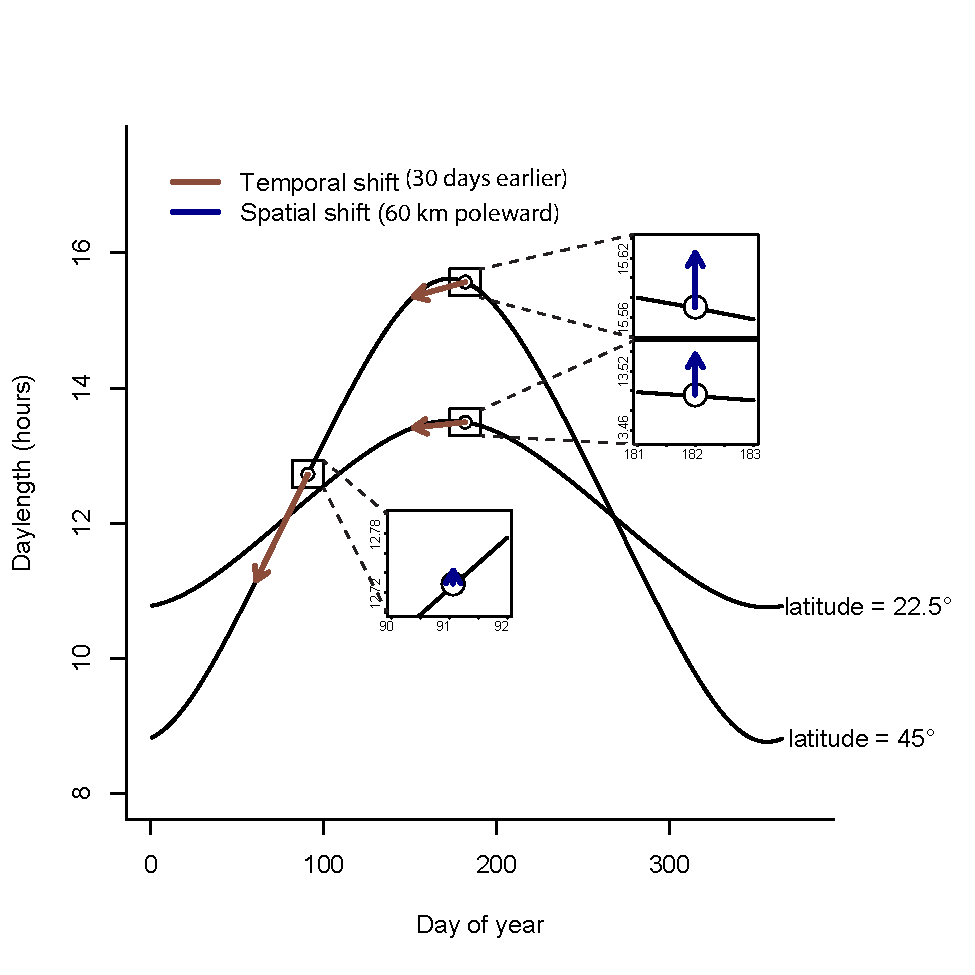
\includegraphics{..//..//analyses/photoperiod/figures/photo_spacetime_v2.pdf} %
\caption{\textbf{Photoperiod varies with latitude and by day of year}, such that temporal shifts in activity yield larger changes in experienced photoperiod compared with spatial shifts. Here, we show this variation at two latitudes (22.5\degree, 45\degree), using hypothetical spatial and temporal shifts. These shifts, which are similar to observed average rates with recent global warming \citep[e.g.,][]{parmesan2006,chen2011}, highlight the greater magnitude in daylength changes close to the equinox (e.g., day of year 91), versus close to the summer solstice (e.g., day of year 182).}
 \label{fig:spacetime}%
 \end{figure}
 
 \begin{figure}[p]
\centering
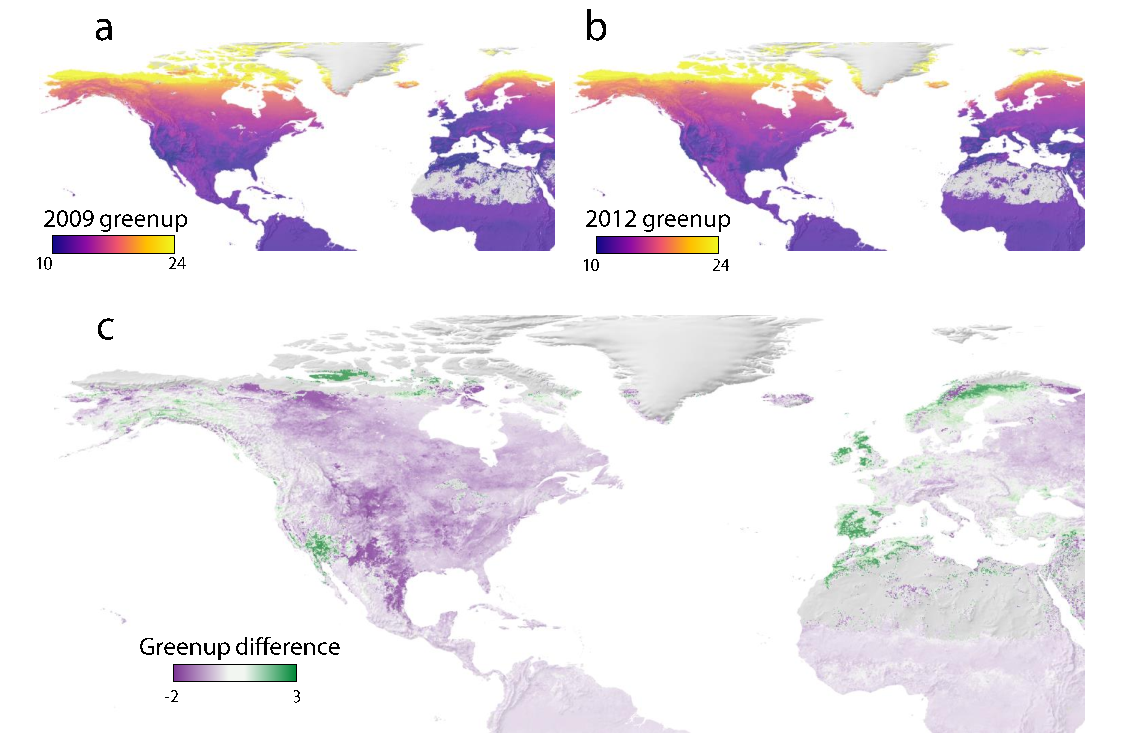
\includegraphics{..//..//docs/photoperiod/figures/Greenup_corr.pdf} %2009 greenup
\caption{\textbf{Photoperiod on the ``green-up" date (i.e., start of spring) varies over space and between years}. Hours of daylight on the date of spring green-up from MODIS satellite data across North America and Europe for an average (2009, a) and  early (2012,b) North American start of spring. The differences between the years (in hours of daylength) are shown in (c).}%Clarify what negative vs. positive means. Again, I would spell out the difference between years in terms of daylength wrt green-up.
 \label{fig:greenup}%
 \end{figure}
 
\begin{figure}[p]
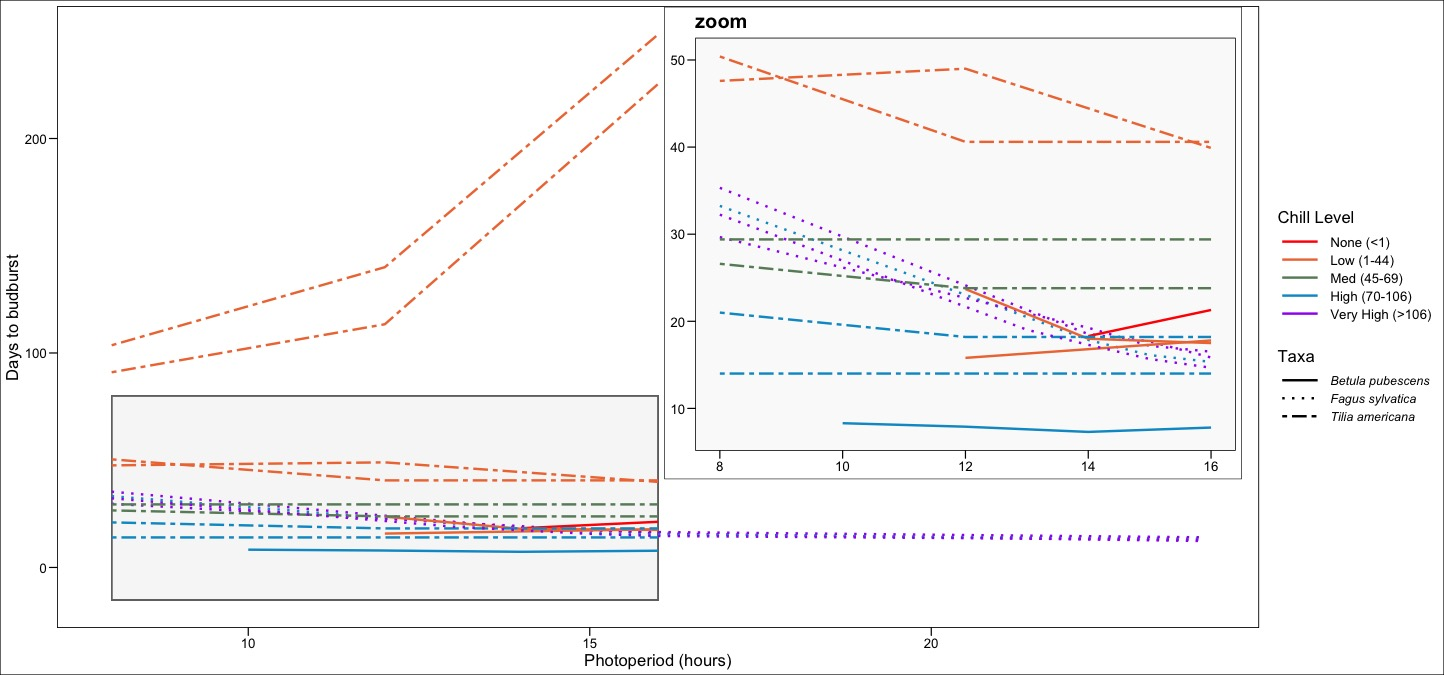
\includegraphics{..//..//analyses/photoperiod/figures/Photo_curv_FINAL.jpeg} 
\caption{\textbf{Nonlinearities in phenological responses to daylength} are apparent in spring woody plant phenology experiments from the OSPREE database, in which three or more photoperiod treatment levels were applied. The shape of the response curves for \textit{Betula pubescens} \citep{Caffarra:2011b}, \textit{Fagus sylvatica} \citep{Heide:1993a} and \textit{Tilia americana} \citep{Ashby:1962aa} differ depending on the amount of winter chilling received (in Chill portions). Species and chilling levels with multiple lines represent plant material from different populations.}
%Note: Hard to tell difference between Tilia and FAgus
%HK: Can you separate figure into 2 graphs? I'd also like to see the zoomed in portion but zoomed out. I find this figure hard to interpret
 \label{fig:photocurve}
 \end{figure}


\begin{figure}[p]
\centering
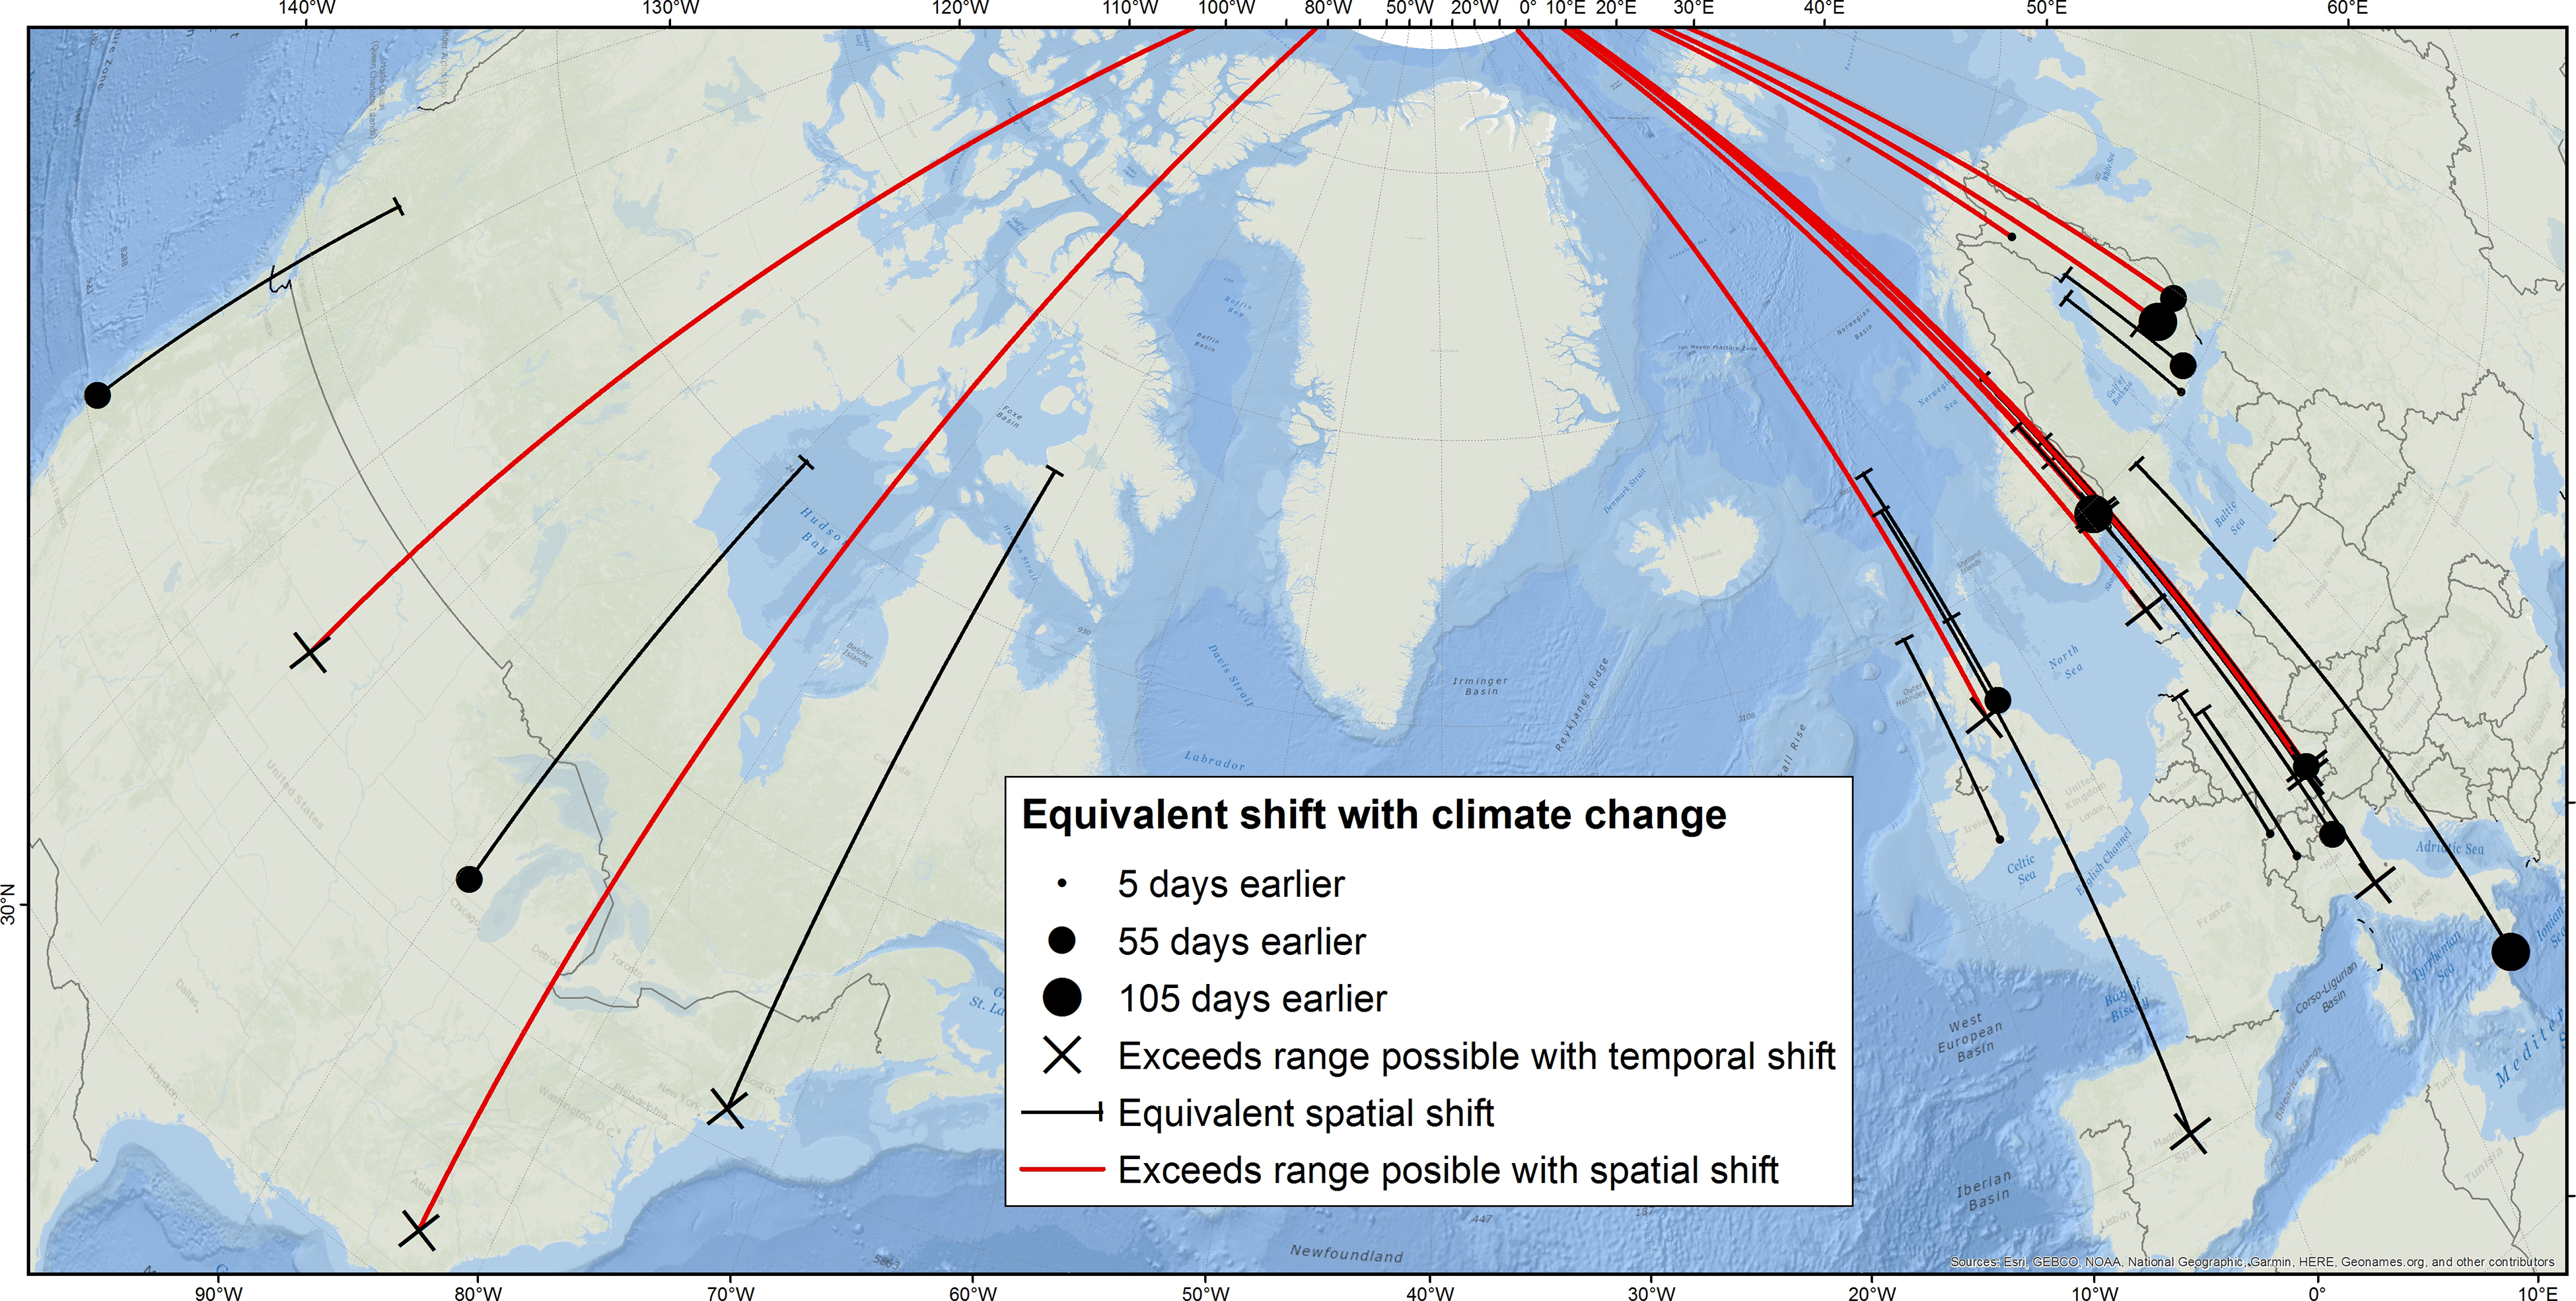
\includegraphics{..//..//analyses/photoperiod/figures/ospree_photopmap_fromblake.jpg} 
\caption{\textbf{Experimental photoperiod treatments and their equivalent spatial and temporal shifts} for experiments in the OSPREE database that manipulate photoperiod. To calculate the required spatial (lines) or temporal (circles and xes) shifts for each experiment, we used observed rates with recent warming: 16.9 kilometers per decade (or approximately 1.5 degrees in 100 years) for spatial shifts (Chen et al. 2011) and 2.3 days per decade (or 23 days in 100 years) for temporal shifts (Parmesan and Yohe 2003).}
 \label{fig:photomap}
 \end{figure}

 
\begin{figure}[p]
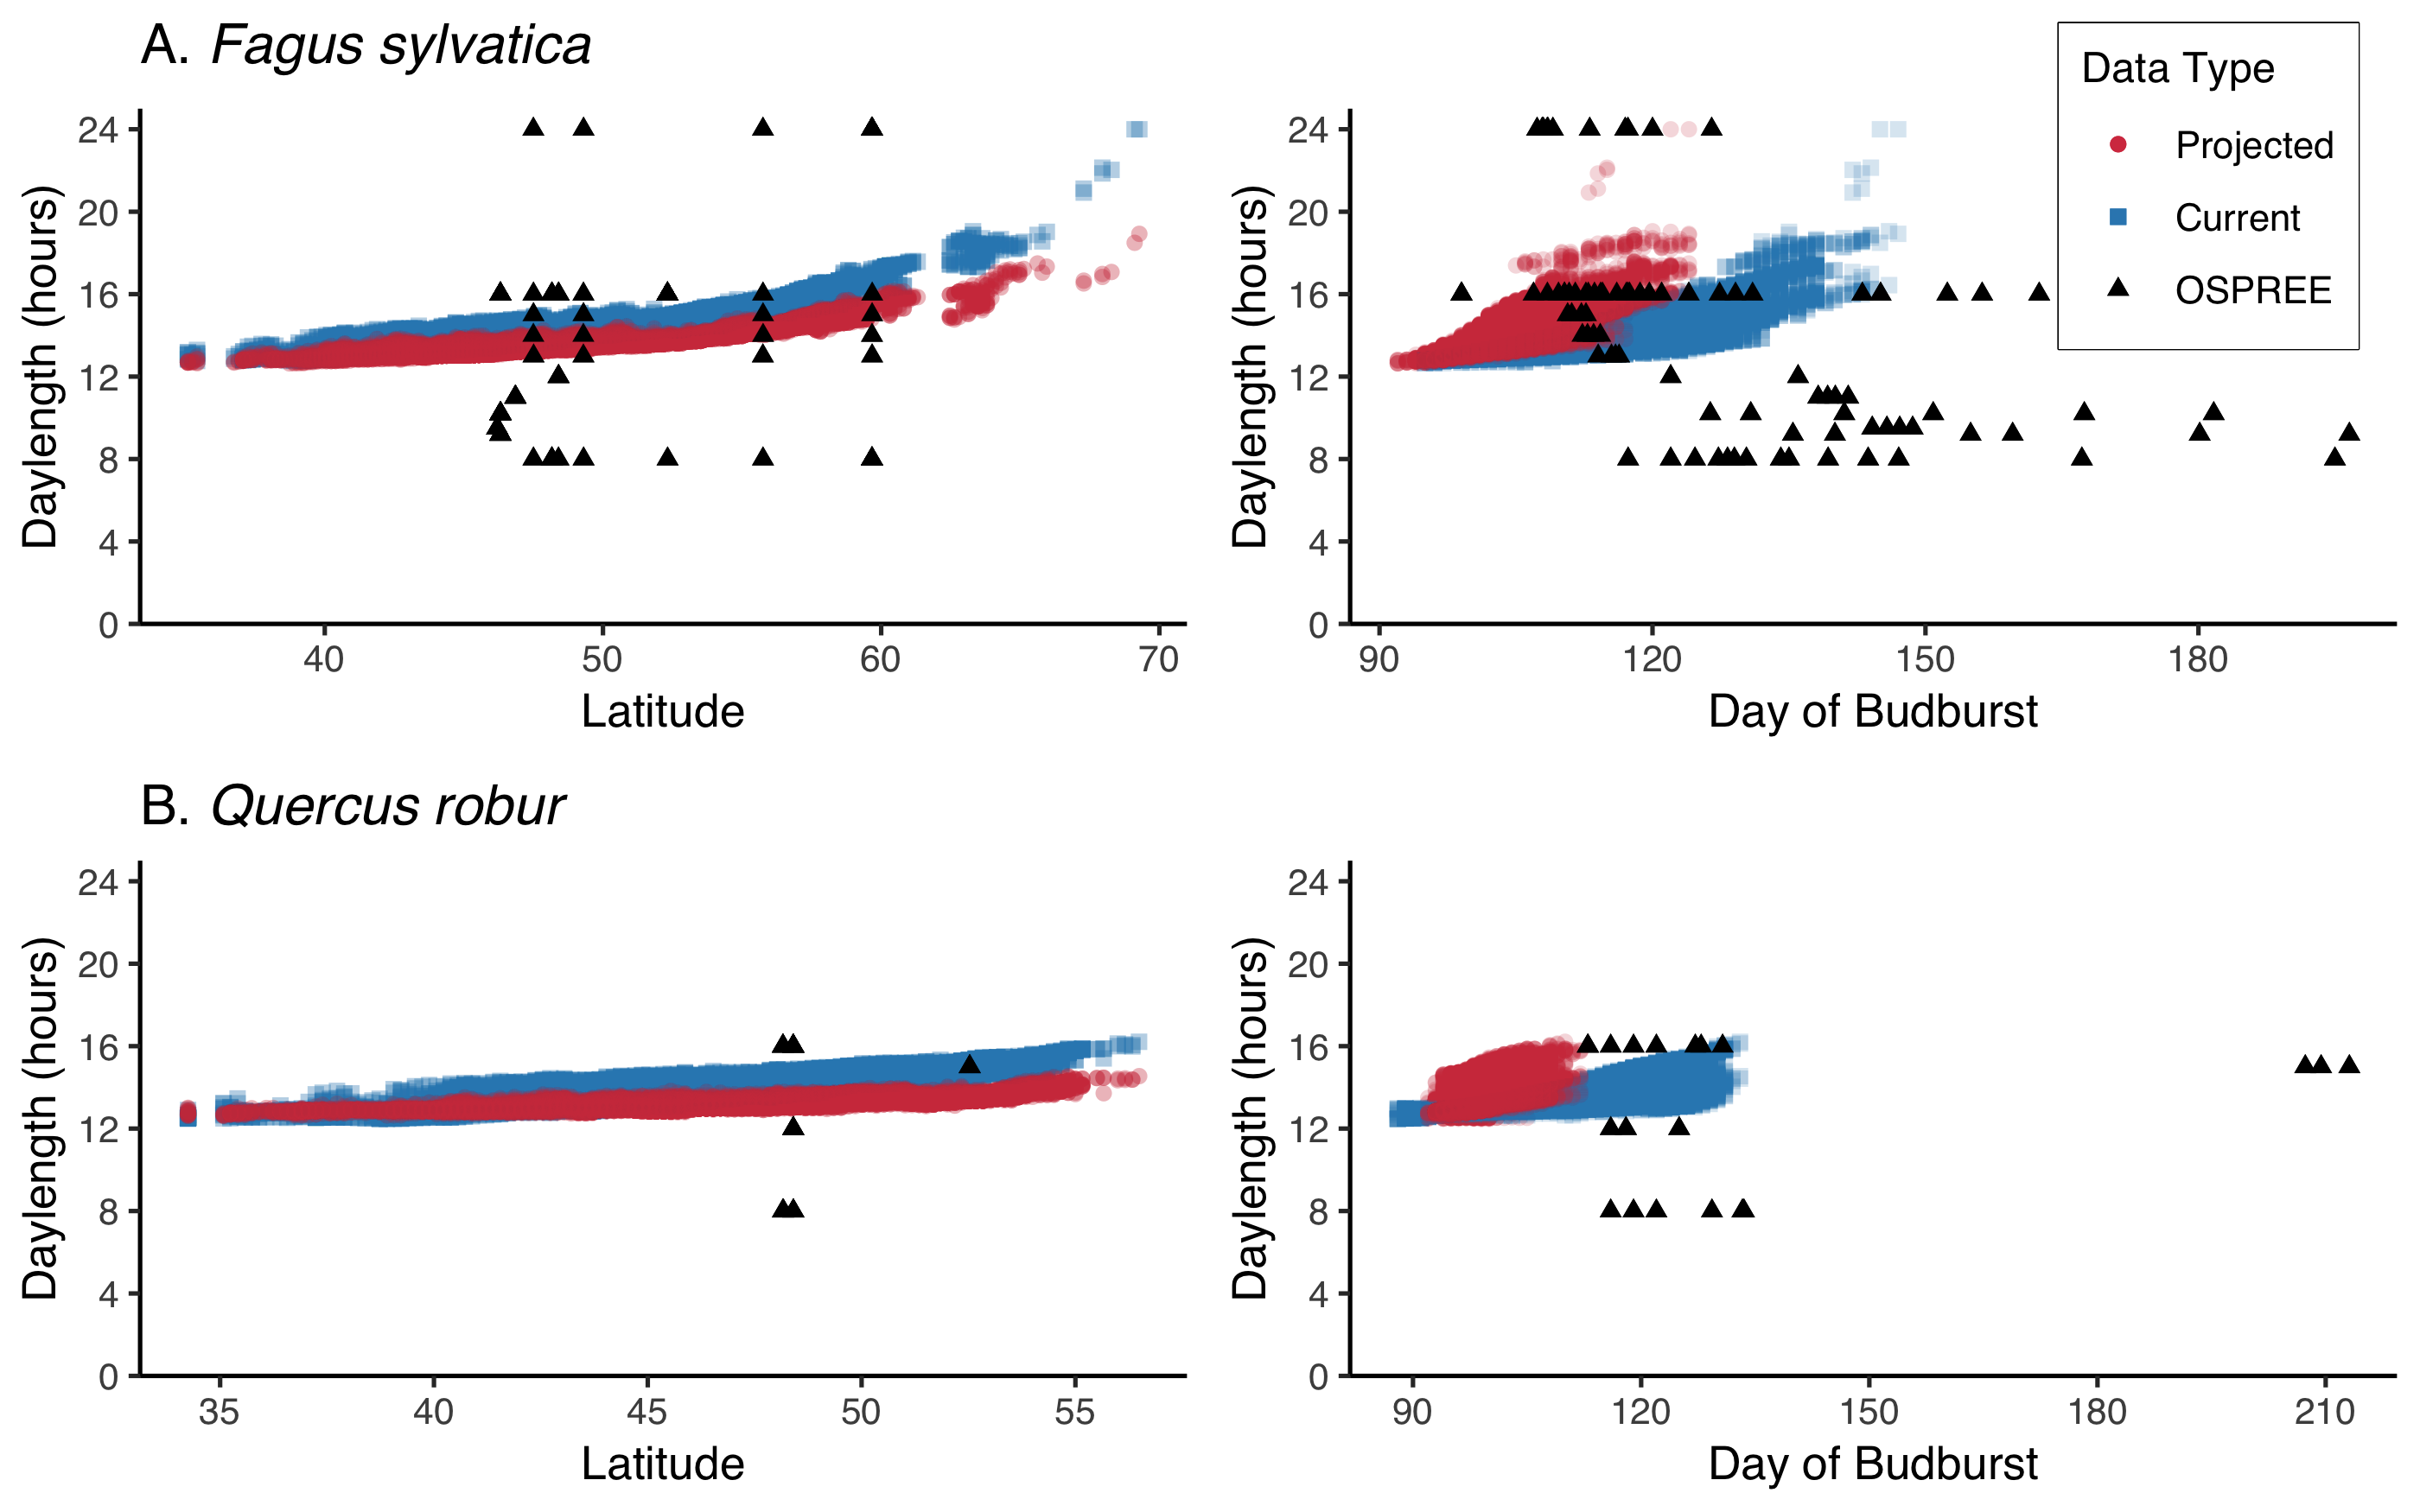
\includegraphics{..//..//analyses/photoperiod/figures/2D_actual_combined.png} 
\caption{\textbf{Experienced photoperiods in experiments differ than those in the natural world}, shown here by latitude (left panels) and by day of budburst (right panels) for \emph{Fagus sylvatica} (A, upper panels) and \emph{Quercus robur} (B, lower panels). Triangles show experimental treatments of photoperiod in the OSPREE database. To illuminate potential gaps between experiments and the natural world, we show the photoperiod when budburst occurs in its current (1981-2000) and projected ranges, \citep[2081-2100, using the A1Fi Phenofit scenario][]{duputie2015}. We scaled the days to budburst for all OSPREE data points by adding the day of budburst from the first Phenofit observation. See Supplemental Materials and \citet{duputie2015} for additional details.} 
 \label{fig:fagus}
 \end{figure}
 
\begin{figure}[p]
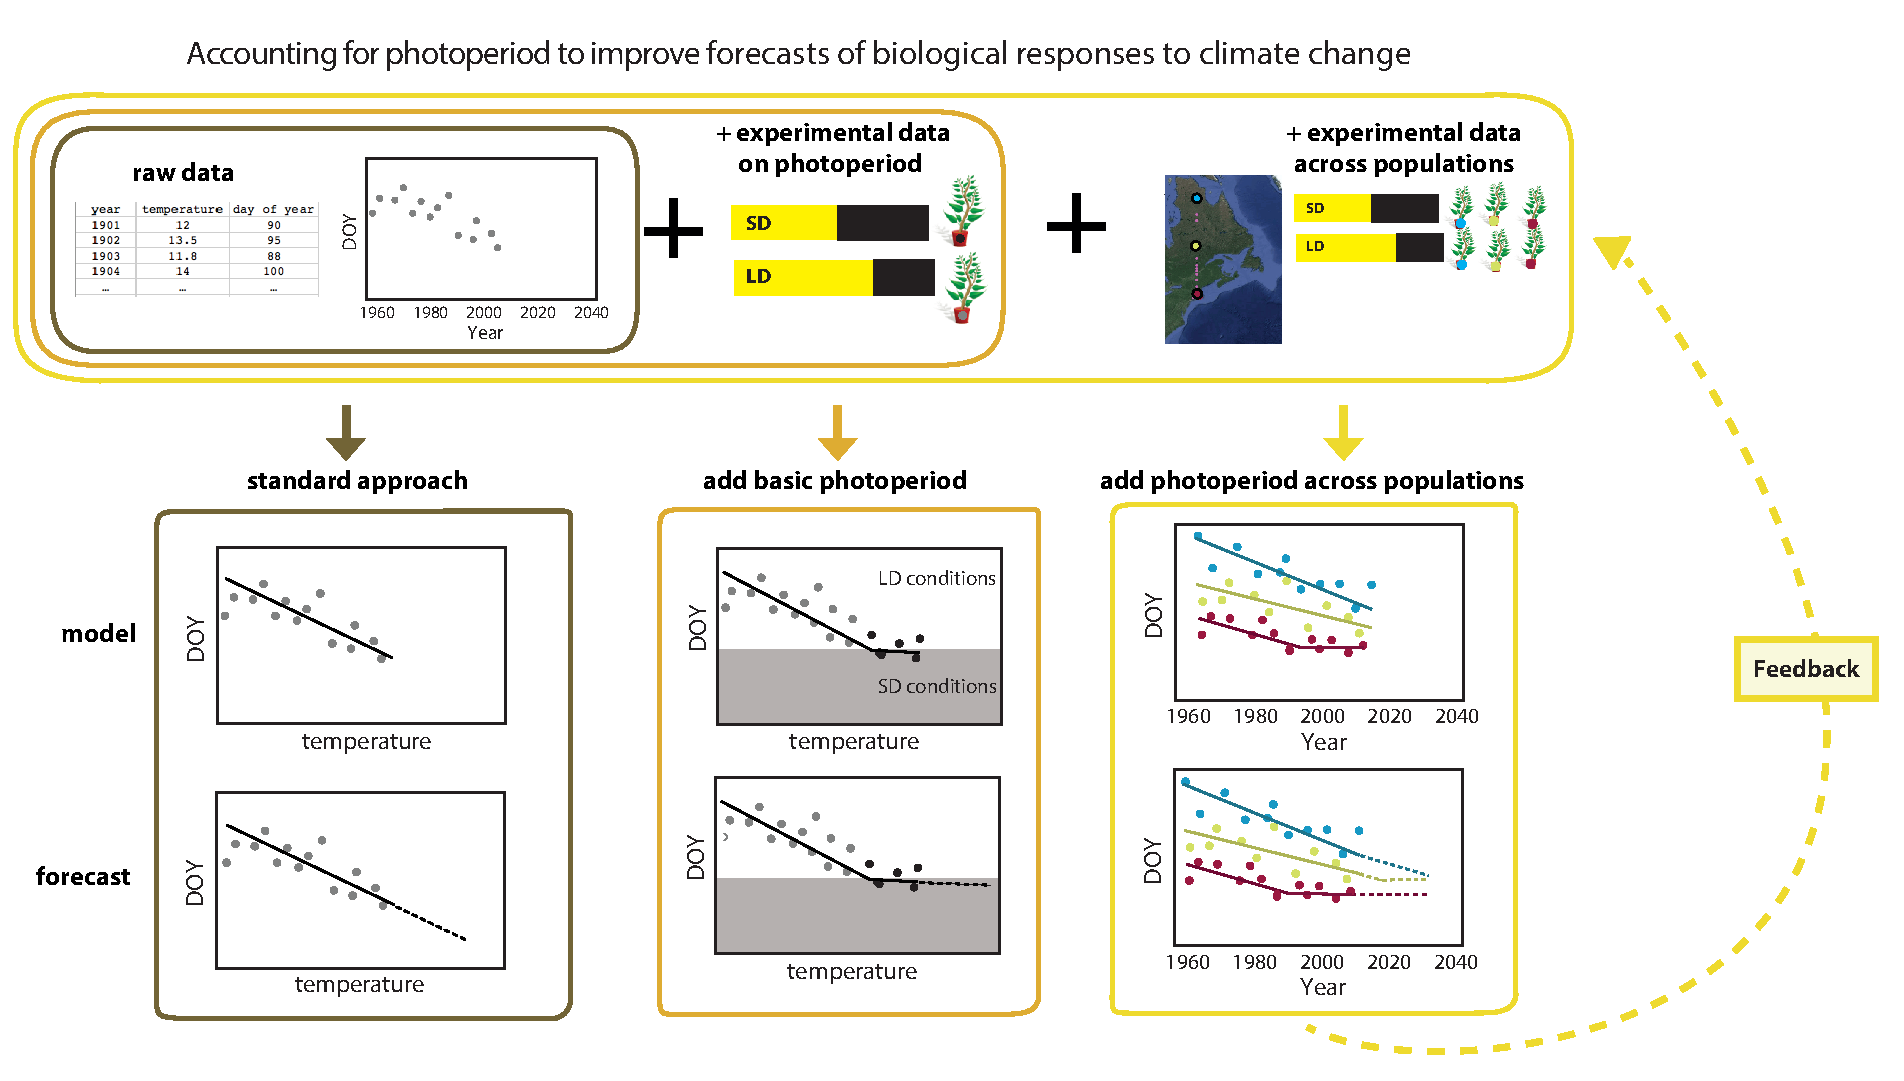
\includegraphics{..//..//analyses/photoperiod/figures/photocondiag6.pdf} 
\caption{\textbf{Conceptual diagram of how to include photoperiod in forecasting biological responses to climate change}. Current approaches for forecasting spring phenology with climate change frequently rely on linear relationships between historical temperature data and observed dates of spring phenology (left panels). Adding responses to photoperiod, which commonly operate as threshold responses to short days (SD) versus long days (LD), will alter these forecasts (center panel) in ways that differ across species that differ in their respective threshold photoperiods. Other factors that interact with photoperiod, such as population-level variation  in photoperiod responses, can be incorporated into forecasts to further improve their accuracy (right panel).}%HK: Because this presents such a good overview, I almost wonder whether you can introduce it before you get into the details of the OSPREE results (i.e. Figure 3-5)?
 \label{fig:condiag}
 \end{figure}
 
 %Other examples of photoperiod control that could be used:
%1.  Onset  and  end  of post-juvenile  moult in migratory warblers and  the  onset  of  autumn  migratory  restlessness  are  advanced in short photoperiods. End  of autumn migratory restlessness, the onset and end of the winter moult  and  the  onset  of  spring  migratory  restlessness  are advanced  by  long  photoperiods. 

%2. temperature and photoperiod control of diapause induction in Lepidoptera https://academic.oup.com/ee/article-abstract/47/5/1314/5032483?redirectedFrom=fulltext

%3. An 1960s review of photoperiod and insect diapause https://www.jstor.org/stable/2459459?seq=1#metadata_info_tab_contents

%A model of a biocontrol insect that includes photoperiod and growing degree days https://www.fs.fed.us/foresthealth/technology/pdfs/BCIP_2013_Grevstad_Proposal.pdf

%Definitely add this paper:
%https://esajournals-onlinelibrary-wiley-com.ezp-prod1.hul.harvard.edu/doi/full/10.1890/14-2071.1

%%%%%%%%%%%%%%%%%%%%%%%%%%%%%%%%%%%%%%%%
\end{document}
%%%%%%%%%%%%%%%%%%%%%%%%%%%%%%%%%%%%%%%%
